\documentclass[1p]{elsarticle_modified}
%\bibliographystyle{elsarticle-num}

%\usepackage[colorlinks]{hyperref}
%\usepackage{abbrmath_seonhwa} %\Abb, \Ascr, \Acal ,\Abf, \Afrak
\usepackage{amsfonts}
\usepackage{amssymb}
\usepackage{amsmath}
\usepackage{amsthm}
\usepackage{scalefnt}
\usepackage{amsbsy}
\usepackage{kotex}
\usepackage{caption}
\usepackage{subfig}
\usepackage{color}
\usepackage{graphicx}
\usepackage{xcolor} %% white, black, red, green, blue, cyan, magenta, yellow
\usepackage{float}
\usepackage{setspace}
\usepackage{hyperref}

\usepackage{tikz}
\usetikzlibrary{arrows}

\usepackage{multirow}
\usepackage{array} % fixed length table
\usepackage{hhline}

%%%%%%%%%%%%%%%%%%%%%
\makeatletter
\renewcommand*\env@matrix[1][\arraystretch]{%
	\edef\arraystretch{#1}%
	\hskip -\arraycolsep
	\let\@ifnextchar\new@ifnextchar
	\array{*\c@MaxMatrixCols c}}
\makeatother %https://tex.stackexchange.com/questions/14071/how-can-i-increase-the-line-spacing-in-a-matrix
%%%%%%%%%%%%%%%

\usepackage[normalem]{ulem}

\newcommand{\msout}[1]{\ifmmode\text{\sout{\ensuremath{#1}}}\else\sout{#1}\fi}
%SOURCE: \msout is \stkout macro in https://tex.stackexchange.com/questions/20609/strikeout-in-math-mode

\newcommand{\cancel}[1]{
	\ifmmode
	{\color{red}\msout{#1}}
	\else
	{\color{red}\sout{#1}}
	\fi
}

\newcommand{\add}[1]{
	{\color{blue}\uwave{#1}}
}

\newcommand{\replace}[2]{
	\ifmmode
	{\color{red}\msout{#1}}{\color{blue}\uwave{#2}}
	\else
	{\color{red}\sout{#1}}{\color{blue}\uwave{#2}}
	\fi
}

\newcommand{\Sol}{\mathcal{S}} %segment
\newcommand{\D}{D} %diagram
\newcommand{\A}{\mathcal{A}} %arc


%%%%%%%%%%%%%%%%%%%%%%%%%%%%%5 test

\def\sl{\operatorname{\textup{SL}}(2,\Cbb)}
\def\psl{\operatorname{\textup{PSL}}(2,\Cbb)}
\def\quan{\mkern 1mu \triangleright \mkern 1mu}

\theoremstyle{definition}
\newtheorem{thm}{Theorem}[section]
\newtheorem{prop}[thm]{Proposition}
\newtheorem{lem}[thm]{Lemma}
\newtheorem{ques}[thm]{Question}
\newtheorem{cor}[thm]{Corollary}
\newtheorem{defn}[thm]{Definition}
\newtheorem{exam}[thm]{Example}
\newtheorem{rmk}[thm]{Remark}
\newtheorem{alg}[thm]{Algorithm}

\newcommand{\I}{\sqrt{-1}}
\begin{document}

%\begin{frontmatter}
%
%\title{Boundary parabolic representations of knots up to 8 crossings}
%
%%% Group authors per affiliation:
%\author{Yunhi Cho} 
%\address{Department of Mathematics, University of Seoul, Seoul, Korea}
%\ead{yhcho@uos.ac.kr}
%
%
%\author{Seonhwa Kim} %\fnref{s_kim}}
%\address{Center for Geometry and Physics, Institute for Basic Science, Pohang, 37673, Korea}
%\ead{ryeona17@ibs.re.kr}
%
%\author{Hyuk Kim}
%\address{Department of Mathematical Sciences, Seoul National University, Seoul 08826, Korea}
%\ead{hyukkim@snu.ac.kr}
%
%\author{Seokbeom Yoon}
%\address{Department of Mathematical Sciences, Seoul National University, Seoul, 08826,  Korea}
%\ead{sbyoon15@snu.ac.kr}
%
%\begin{abstract}
%We find all boundary parabolic representation of knots up to 8 crossings.
%
%\end{abstract}
%\begin{keyword}
%    \MSC[2010] 57M25 
%\end{keyword}
%
%\end{frontmatter}

%\linenumbers
%\tableofcontents
%
\newcommand\colored[1]{\textcolor{white}{\rule[-0.35ex]{0.8em}{1.4ex}}\kern-0.8em\color{red} #1}%
%\newcommand\colored[1]{\textcolor{white}{ #1}\kern-2.17ex	\textcolor{white}{ #1}\kern-1.81ex	\textcolor{white}{ #1}\kern-2.15ex\color{red}#1	}

{\Large $\underline{11a_{326}~(K11a_{326})}$}

\setlength{\tabcolsep}{10pt}
\renewcommand{\arraystretch}{1.6}
\vspace{1cm}\begin{tabular}{m{100pt}>{\centering\arraybackslash}m{274pt}}
\multirow{5}{120pt}{
	\centering
	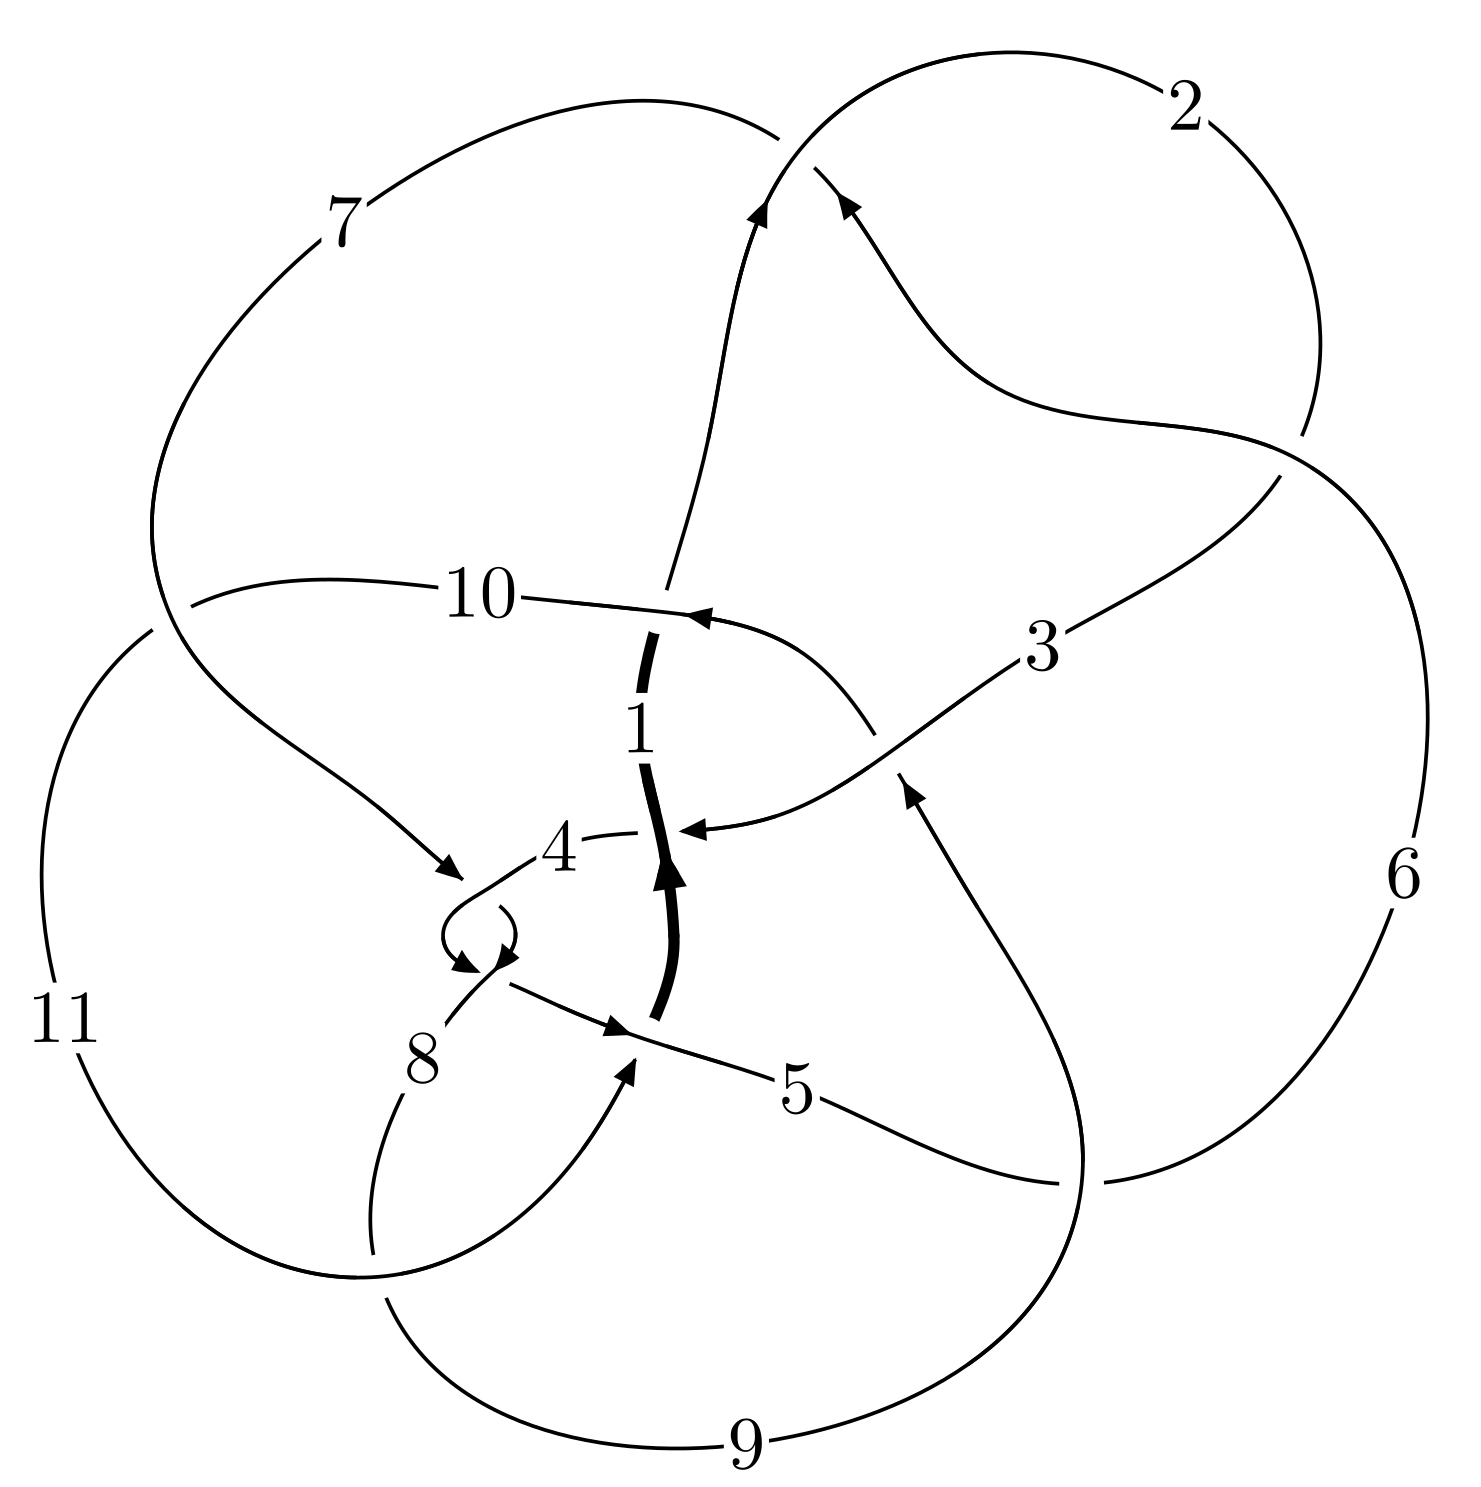
\includegraphics[width=112pt]{../../../GIT/diagram.site/Diagrams/png/575_11a_326.png}\\
\ \ \ A knot diagram\footnotemark}&
\allowdisplaybreaks
\textbf{Linearized knot diagam} \\
\cline{2-2}
 &
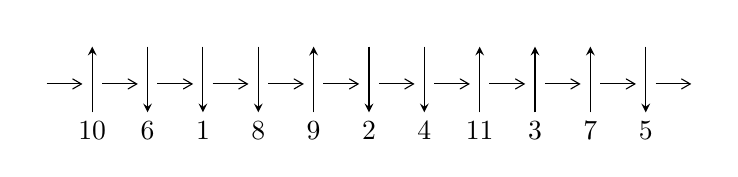
\begin{tikzpicture}[x=20pt, y=17pt]
	% nodes
	\node (C0) at (0, 0) {};
	\node (C1) at (1, 0) {};
	\node (C1U) at (1, +1) {};
	\node (C1D) at (1, -1) {10};

	\node (C2) at (2, 0) {};
	\node (C2U) at (2, +1) {};
	\node (C2D) at (2, -1) {6};

	\node (C3) at (3, 0) {};
	\node (C3U) at (3, +1) {};
	\node (C3D) at (3, -1) {1};

	\node (C4) at (4, 0) {};
	\node (C4U) at (4, +1) {};
	\node (C4D) at (4, -1) {8};

	\node (C5) at (5, 0) {};
	\node (C5U) at (5, +1) {};
	\node (C5D) at (5, -1) {9};

	\node (C6) at (6, 0) {};
	\node (C6U) at (6, +1) {};
	\node (C6D) at (6, -1) {2};

	\node (C7) at (7, 0) {};
	\node (C7U) at (7, +1) {};
	\node (C7D) at (7, -1) {4};

	\node (C8) at (8, 0) {};
	\node (C8U) at (8, +1) {};
	\node (C8D) at (8, -1) {11};

	\node (C9) at (9, 0) {};
	\node (C9U) at (9, +1) {};
	\node (C9D) at (9, -1) {3};

	\node (C10) at (10, 0) {};
	\node (C10U) at (10, +1) {};
	\node (C10D) at (10, -1) {7};

	\node (C11) at (11, 0) {};
	\node (C11U) at (11, +1) {};
	\node (C11D) at (11, -1) {5};
	\node (C12) at (12, 0) {};

	% arrows
	\draw[->,>={angle 60}]
	(C0) edge (C1) (C1) edge (C2) (C2) edge (C3) (C3) edge (C4) (C4) edge (C5) (C5) edge (C6) (C6) edge (C7) (C7) edge (C8) (C8) edge (C9) (C9) edge (C10) (C10) edge (C11) (C11) edge (C12) ;	\draw[->,>=stealth]
	(C1D) edge (C1U) (C2U) edge (C2D) (C3U) edge (C3D) (C4U) edge (C4D) (C5D) edge (C5U) (C6U) edge (C6D) (C7U) edge (C7D) (C8D) edge (C8U) (C9D) edge (C9U) (C10D) edge (C10U) (C11U) edge (C11D) ;
	\end{tikzpicture} \\
\hhline{~~} \\& 
\textbf{Solving Sequence} \\ \cline{2-2} 
 &
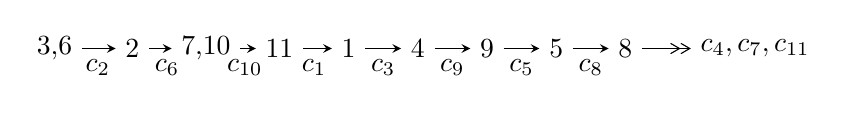
\begin{tikzpicture}[x=25pt, y=7pt]
	% node
	\node (A0) at (-1/8, 0) {3,6};
	\node (A1) at (1, 0) {2};
	\node (A2) at (33/16, 0) {7,10};
	\node (A3) at (25/8, 0) {11};
	\node (A4) at (33/8, 0) {1};
	\node (A5) at (41/8, 0) {4};
	\node (A6) at (49/8, 0) {9};
	\node (A7) at (57/8, 0) {5};
	\node (A8) at (65/8, 0) {8};
	\node (C1) at (1/2, -1) {$c_{2}$};
	\node (C2) at (3/2, -1) {$c_{6}$};
	\node (C3) at (21/8, -1) {$c_{10}$};
	\node (C4) at (29/8, -1) {$c_{1}$};
	\node (C5) at (37/8, -1) {$c_{3}$};
	\node (C6) at (45/8, -1) {$c_{9}$};
	\node (C7) at (53/8, -1) {$c_{5}$};
	\node (C8) at (61/8, -1) {$c_{8}$};
	\node (A9) at (10, 0) {$c_{4},c_{7},c_{11}$};

	% edge
	\draw[->,>=stealth]	
	(A0) edge (A1) (A1) edge (A2) (A2) edge (A3) (A3) edge (A4) (A4) edge (A5) (A5) edge (A6) (A6) edge (A7) (A7) edge (A8) ;
	\draw[->>,>={angle 60}]	
	(A8) edge (A9);
\end{tikzpicture} \\ 

\end{tabular} \\

\footnotetext{
The image of knot diagram is generated by the software ``\textbf{Draw programme}" developed by Andrew Bartholomew(\url{http://www.layer8.co.uk/maths/draw/index.htm\#Running-draw}), where we modified some parts for our purpose(\url{https://github.com/CATsTAILs/LinksPainter}).
}\phantom \\ \newline 
\centering \textbf{Ideals for irreducible components\footnotemark of $X_{\text{par}}$} 
 
\begin{align*}
I^u_{1}&=\langle 
-1.39236\times10^{318} u^{105}-4.25978\times10^{318} u^{104}+\cdots+4.43640\times10^{318} b-1.00560\times10^{319},\\
\phantom{I^u_{1}}&\phantom{= \langle  }-7.92637\times10^{317} u^{105}-2.62180\times10^{318} u^{104}+\cdots+3.41262\times10^{317} a-1.84851\times10^{318},\\
\phantom{I^u_{1}}&\phantom{= \langle  }u^{106}+3 u^{105}+\cdots+19 u-1\rangle \\
I^u_{2}&=\langle 
311058123 u^{21}-50616715 u^{20}+\cdots+462381937 b-8437483,\\
\phantom{I^u_{2}}&\phantom{= \langle  }616215260 u^{21}+9916634 u^{20}+\cdots+462381937 a+572933757,\;u^{22}+6 u^{20}+\cdots+3 u-1\rangle \\
\\
\end{align*}
\raggedright * 2 irreducible components of $\dim_{\mathbb{C}}=0$, with total 128 representations.\\
\footnotetext{All coefficients of polynomials are rational numbers. But the coefficients are sometimes approximated in decimal forms when there is not enough margin.}
\newpage
\renewcommand{\arraystretch}{1}
\centering \section*{I. $I^u_{1}= \langle -1.39\times10^{318} u^{105}-4.26\times10^{318} u^{104}+\cdots+4.44\times10^{318} b-1.01\times10^{319},\;-7.93\times10^{317} u^{105}-2.62\times10^{318} u^{104}+\cdots+3.41\times10^{317} a-1.85\times10^{318},\;u^{106}+3 u^{105}+\cdots+19 u-1 \rangle$}
\flushleft \textbf{(i) Arc colorings}\\
\begin{tabular}{m{7pt} m{180pt} m{7pt} m{180pt} }
\flushright $a_{3}=$&$\begin{pmatrix}1\\0\end{pmatrix}$ \\
\flushright $a_{6}=$&$\begin{pmatrix}0\\u\end{pmatrix}$ \\
\flushright $a_{2}=$&$\begin{pmatrix}1\\- u^2\end{pmatrix}$ \\
\flushright $a_{7}=$&$\begin{pmatrix}- u\\u^3+u\end{pmatrix}$ \\
\flushright $a_{10}=$&$\begin{pmatrix}2.32267 u^{105}+7.68268 u^{104}+\cdots-77.0561 u+5.41671\\0.313848 u^{105}+0.960189 u^{104}+\cdots-28.1503 u+2.26670\end{pmatrix}$ \\
\flushright $a_{11}=$&$\begin{pmatrix}1.94720 u^{105}+6.49173 u^{104}+\cdots-80.8911 u+5.76853\\0.0903806 u^{105}+0.134570 u^{104}+\cdots-25.1663 u+1.97942\end{pmatrix}$ \\
\flushright $a_{1}=$&$\begin{pmatrix}0.536095 u^{105}+0.763638 u^{104}+\cdots-218.875 u+17.7105\\0.0757890 u^{105}+0.130522 u^{104}+\cdots-27.0376 u+2.47019\end{pmatrix}$ \\
\flushright $a_{4}=$&$\begin{pmatrix}1.74444 u^{105}+5.31471 u^{104}+\cdots-231.801 u+15.2966\\0.636229 u^{105}+2.00879 u^{104}+\cdots-43.7176 u+2.69763\end{pmatrix}$ \\
\flushright $a_{9}=$&$\begin{pmatrix}2.00882 u^{105}+6.72249 u^{104}+\cdots-48.9057 u+3.15001\\0.313848 u^{105}+0.960189 u^{104}+\cdots-28.1503 u+2.26670\end{pmatrix}$ \\
\flushright $a_{5}=$&$\begin{pmatrix}-1.45668 u^{105}-4.17549 u^{104}+\cdots+45.8949 u-8.57048\\-0.300360 u^{105}-1.16893 u^{104}+\cdots-4.12988 u-0.387022\end{pmatrix}$ \\
\flushright $a_{8}=$&$\begin{pmatrix}-0.131397 u^{105}+0.259568 u^{104}+\cdots+251.587 u-13.5190\\-0.400537 u^{105}-1.31079 u^{104}+\cdots+39.8917 u-2.14966\end{pmatrix}$\\ \flushright $a_{8}=$&$\begin{pmatrix}-0.131397 u^{105}+0.259568 u^{104}+\cdots+251.587 u-13.5190\\-0.400537 u^{105}-1.31079 u^{104}+\cdots+39.8917 u-2.14966\end{pmatrix}$\\&\end{tabular}
\flushleft \textbf{(ii) Obstruction class $= -1$}\\~\\
\flushleft \textbf{(iii) Cusp Shapes $= 0.235617 u^{105}+1.09038 u^{104}+\cdots-71.7333 u+9.44104$}\\~\\
\newpage\renewcommand{\arraystretch}{1}
\flushleft \textbf{(iv) u-Polynomials at the component}\newline \\
\begin{tabular}{m{50pt}|m{274pt}}
Crossings & \hspace{64pt}u-Polynomials at each crossing \\
\hline $$\begin{aligned}c_{1}\end{aligned}$$&$\begin{aligned}
&u^{106}-8 u^{105}+\cdots+8867 u-3445
\end{aligned}$\\
\hline $$\begin{aligned}c_{2},c_{6}\end{aligned}$$&$\begin{aligned}
&u^{106}+3 u^{105}+\cdots+19 u-1
\end{aligned}$\\
\hline $$\begin{aligned}c_{3}\end{aligned}$$&$\begin{aligned}
&u^{106}-10 u^{105}+\cdots-35874 u+5203
\end{aligned}$\\
\hline $$\begin{aligned}c_{4},c_{7}\end{aligned}$$&$\begin{aligned}
&u^{106}-36 u^{104}+\cdots+191 u-11
\end{aligned}$\\
\hline $$\begin{aligned}c_{5}\end{aligned}$$&$\begin{aligned}
&u^{106}-4 u^{105}+\cdots-9831064 u+2445611
\end{aligned}$\\
\hline $$\begin{aligned}c_{8}\end{aligned}$$&$\begin{aligned}
&u^{106}-4 u^{105}+\cdots-31 u-1
\end{aligned}$\\
\hline $$\begin{aligned}c_{9}\end{aligned}$$&$\begin{aligned}
&u^{106}-19 u^{104}+\cdots-97525 u-19379
\end{aligned}$\\
\hline $$\begin{aligned}c_{10}\end{aligned}$$&$\begin{aligned}
&u^{106}-22 u^{104}+\cdots+40099 u+4897
\end{aligned}$\\
\hline $$\begin{aligned}c_{11}\end{aligned}$$&$\begin{aligned}
&u^{106}+2 u^{105}+\cdots-5 u+1
\end{aligned}$\\
\hline
\end{tabular}\\~\\
\newpage\renewcommand{\arraystretch}{1}
\flushleft \textbf{(v) Riley Polynomials at the component}\newline \\
\begin{tabular}{m{50pt}|m{274pt}}
Crossings & \hspace{64pt}Riley Polynomials at each crossing \\
\hline $$\begin{aligned}c_{1}\end{aligned}$$&$\begin{aligned}
&y^{106}-26 y^{105}+\cdots-349655619 y+11868025
\end{aligned}$\\
\hline $$\begin{aligned}c_{2},c_{6}\end{aligned}$$&$\begin{aligned}
&y^{106}+73 y^{105}+\cdots+93 y+1
\end{aligned}$\\
\hline $$\begin{aligned}c_{3}\end{aligned}$$&$\begin{aligned}
&y^{106}+12 y^{105}+\cdots+307328166 y+27071209
\end{aligned}$\\
\hline $$\begin{aligned}c_{4},c_{7}\end{aligned}$$&$\begin{aligned}
&y^{106}-72 y^{105}+\cdots-20795 y+121
\end{aligned}$\\
\hline $$\begin{aligned}c_{5}\end{aligned}$$&$\begin{aligned}
&y^{106}-62 y^{105}+\cdots-243034883661070 y+5981013163321
\end{aligned}$\\
\hline $$\begin{aligned}c_{8}\end{aligned}$$&$\begin{aligned}
&y^{106}-8 y^{105}+\cdots-345 y+1
\end{aligned}$\\
\hline $$\begin{aligned}c_{9}\end{aligned}$$&$\begin{aligned}
&y^{106}-38 y^{105}+\cdots-3790134761 y+375545641
\end{aligned}$\\
\hline $$\begin{aligned}c_{10}\end{aligned}$$&$\begin{aligned}
&y^{106}-44 y^{105}+\cdots-2051676353 y+23980609
\end{aligned}$\\
\hline $$\begin{aligned}c_{11}\end{aligned}$$&$\begin{aligned}
&y^{106}+84 y^{104}+\cdots-7 y+1
\end{aligned}$\\
\hline
\end{tabular}\\~\\
\newpage\flushleft \textbf{(vi) Complex Volumes and Cusp Shapes}
$$\begin{array}{c|c|c}  
\text{Solutions to }I^u_{1}& \I (\text{vol} + \sqrt{-1}CS) & \text{Cusp shape}\\
 \hline 
\begin{aligned}
u &= \phantom{-}0.004504 + 0.988733 I \\
a &= \phantom{-}0.315079 + 0.330456 I \\
b &= \phantom{-}0.50078 + 1.51754 I\end{aligned}
 & -1.37131 + 2.82623 I & \phantom{-0.000000 } 0 \\ \hline\begin{aligned}
u &= \phantom{-}0.004504 - 0.988733 I \\
a &= \phantom{-}0.315079 - 0.330456 I \\
b &= \phantom{-}0.50078 - 1.51754 I\end{aligned}
 & -1.37131 - 2.82623 I & \phantom{-0.000000 } 0 \\ \hline\begin{aligned}
u &= -0.988852 + 0.225632 I \\
a &= \phantom{-}0.526268 + 0.083150 I \\
b &= -0.571986 - 0.392628 I\end{aligned}
 & -2.95995 + 0.48399 I & \phantom{-0.000000 } 0 \\ \hline\begin{aligned}
u &= -0.988852 - 0.225632 I \\
a &= \phantom{-}0.526268 - 0.083150 I \\
b &= -0.571986 + 0.392628 I\end{aligned}
 & -2.95995 - 0.48399 I & \phantom{-0.000000 } 0 \\ \hline\begin{aligned}
u &= \phantom{-}1.009820 + 0.111821 I \\
a &= \phantom{-}0.138217 + 0.405761 I \\
b &= \phantom{-}0.954539 + 0.430058 I\end{aligned}
 & \phantom{-}0.96920 + 3.40112 I & \phantom{-0.000000 } 0 \\ \hline\begin{aligned}
u &= \phantom{-}1.009820 - 0.111821 I \\
a &= \phantom{-}0.138217 - 0.405761 I \\
b &= \phantom{-}0.954539 - 0.430058 I\end{aligned}
 & \phantom{-}0.96920 - 3.40112 I & \phantom{-0.000000 } 0 \\ \hline\begin{aligned}
u &= \phantom{-}0.175510 + 0.953433 I \\
a &= -1.51425 - 0.81029 I \\
b &= -0.389599 - 0.483666 I\end{aligned}
 & \phantom{-}2.89668 - 0.78297 I & \phantom{-0.000000 } 0 \\ \hline\begin{aligned}
u &= \phantom{-}0.175510 - 0.953433 I \\
a &= -1.51425 + 0.81029 I \\
b &= -0.389599 + 0.483666 I\end{aligned}
 & \phantom{-}2.89668 + 0.78297 I & \phantom{-0.000000 } 0 \\ \hline\begin{aligned}
u &= -0.374861 + 0.992057 I \\
a &= -2.21826 + 0.55212 I \\
b &= -1.99480 - 0.51836 I\end{aligned}
 & -0.83829 + 8.68306 I & \phantom{-0.000000 } 0 \\ \hline\begin{aligned}
u &= -0.374861 - 0.992057 I \\
a &= -2.21826 - 0.55212 I \\
b &= -1.99480 + 0.51836 I\end{aligned}
 & -0.83829 - 8.68306 I & \phantom{-0.000000 } 0\\
 \hline 
 \end{array}$$\newpage$$\begin{array}{c|c|c}  
\text{Solutions to }I^u_{1}& \I (\text{vol} + \sqrt{-1}CS) & \text{Cusp shape}\\
 \hline 
\begin{aligned}
u &= \phantom{-}0.432345 + 0.999010 I \\
a &= \phantom{-}0.865851 + 0.039909 I \\
b &= \phantom{-}0.902968 - 1.032280 I\end{aligned}
 & \phantom{-}0.74617 - 3.75338 I & \phantom{-0.000000 } 0 \\ \hline\begin{aligned}
u &= \phantom{-}0.432345 - 0.999010 I \\
a &= \phantom{-}0.865851 - 0.039909 I \\
b &= \phantom{-}0.902968 + 1.032280 I\end{aligned}
 & \phantom{-}0.74617 + 3.75338 I & \phantom{-0.000000 } 0 \\ \hline\begin{aligned}
u &= \phantom{-}0.016823 + 0.887495 I \\
a &= -1.97243 + 1.45010 I \\
b &= -0.975184 + 0.646919 I\end{aligned}
 & -1.63192 - 3.20943 I & \phantom{-0.000000 } 0 \\ \hline\begin{aligned}
u &= \phantom{-}0.016823 - 0.887495 I \\
a &= -1.97243 - 1.45010 I \\
b &= -0.975184 - 0.646919 I\end{aligned}
 & -1.63192 + 3.20943 I & \phantom{-0.000000 } 0 \\ \hline\begin{aligned}
u &= \phantom{-}0.398783 + 1.042840 I \\
a &= \phantom{-}1.58801 - 0.16903 I \\
b &= \phantom{-}0.659942 - 0.624132 I\end{aligned}
 & -3.88026 - 0.66373 I & \phantom{-0.000000 } 0 \\ \hline\begin{aligned}
u &= \phantom{-}0.398783 - 1.042840 I \\
a &= \phantom{-}1.58801 + 0.16903 I \\
b &= \phantom{-}0.659942 + 0.624132 I\end{aligned}
 & -3.88026 + 0.66373 I & \phantom{-0.000000 } 0 \\ \hline\begin{aligned}
u &= \phantom{-}0.801015 + 0.368704 I \\
a &= \phantom{-}0.809671 - 0.532522 I \\
b &= -0.097040 - 0.678675 I\end{aligned}
 & -1.18628 - 0.97362 I & \phantom{-0.000000 } 0 \\ \hline\begin{aligned}
u &= \phantom{-}0.801015 - 0.368704 I \\
a &= \phantom{-}0.809671 + 0.532522 I \\
b &= -0.097040 + 0.678675 I\end{aligned}
 & -1.18628 + 0.97362 I & \phantom{-0.000000 } 0 \\ \hline\begin{aligned}
u &= -0.701103 + 0.525072 I \\
a &= \phantom{-}0.191668 - 1.088290 I \\
b &= \phantom{-}1.120550 - 0.725615 I\end{aligned}
 & -2.25902 - 4.46440 I & \phantom{-0.000000 } 0 \\ \hline\begin{aligned}
u &= -0.701103 - 0.525072 I \\
a &= \phantom{-}0.191668 + 1.088290 I \\
b &= \phantom{-}1.120550 + 0.725615 I\end{aligned}
 & -2.25902 + 4.46440 I & \phantom{-0.000000 } 0\\
 \hline 
 \end{array}$$\newpage$$\begin{array}{c|c|c}  
\text{Solutions to }I^u_{1}& \I (\text{vol} + \sqrt{-1}CS) & \text{Cusp shape}\\
 \hline 
\begin{aligned}
u &= -0.692760 + 0.496513 I \\
a &= \phantom{-}0.078806 + 0.123174 I \\
b &= \phantom{-}0.509835 + 0.878093 I\end{aligned}
 & -1.04735 + 4.26740 I & \phantom{-0.000000 } 0 \\ \hline\begin{aligned}
u &= -0.692760 - 0.496513 I \\
a &= \phantom{-}0.078806 - 0.123174 I \\
b &= \phantom{-}0.509835 - 0.878093 I\end{aligned}
 & -1.04735 - 4.26740 I & \phantom{-0.000000 } 0 \\ \hline\begin{aligned}
u &= \phantom{-}0.095837 + 1.144680 I \\
a &= \phantom{-}0.86253 + 1.42437 I \\
b &= \phantom{-}0.510950 - 0.540666 I\end{aligned}
 & \phantom{-}5.27080 - 3.32416 I & \phantom{-0.000000 } 0 \\ \hline\begin{aligned}
u &= \phantom{-}0.095837 - 1.144680 I \\
a &= \phantom{-}0.86253 - 1.42437 I \\
b &= \phantom{-}0.510950 + 0.540666 I\end{aligned}
 & \phantom{-}5.27080 + 3.32416 I & \phantom{-0.000000 } 0 \\ \hline\begin{aligned}
u &= -0.023574 + 1.153230 I \\
a &= -1.40824 - 0.41746 I \\
b &= -0.90634 - 1.37571 I\end{aligned}
 & \phantom{-}4.45667 - 0.16513 I & \phantom{-0.000000 } 0 \\ \hline\begin{aligned}
u &= -0.023574 - 1.153230 I \\
a &= -1.40824 + 0.41746 I \\
b &= -0.90634 + 1.37571 I\end{aligned}
 & \phantom{-}4.45667 + 0.16513 I & \phantom{-0.000000 } 0 \\ \hline\begin{aligned}
u &= \phantom{-}0.357793 + 1.097090 I \\
a &= \phantom{-}2.14597 + 0.07710 I \\
b &= \phantom{-}0.567709 - 0.622795 I\end{aligned}
 & -0.75293 - 9.92335 I & \phantom{-0.000000 } 0 \\ \hline\begin{aligned}
u &= \phantom{-}0.357793 - 1.097090 I \\
a &= \phantom{-}2.14597 - 0.07710 I \\
b &= \phantom{-}0.567709 + 0.622795 I\end{aligned}
 & -0.75293 + 9.92335 I & \phantom{-0.000000 } 0 \\ \hline\begin{aligned}
u &= \phantom{-}0.758523 + 0.371148 I \\
a &= -0.1018870 + 0.0081553 I \\
b &= -0.199249 - 0.990047 I\end{aligned}
 & -5.96051 - 3.62479 I & \phantom{-0.000000 } 0 \\ \hline\begin{aligned}
u &= \phantom{-}0.758523 - 0.371148 I \\
a &= -0.1018870 - 0.0081553 I \\
b &= -0.199249 + 0.990047 I\end{aligned}
 & -5.96051 + 3.62479 I & \phantom{-0.000000 } 0\\
 \hline 
 \end{array}$$\newpage$$\begin{array}{c|c|c}  
\text{Solutions to }I^u_{1}& \I (\text{vol} + \sqrt{-1}CS) & \text{Cusp shape}\\
 \hline 
\begin{aligned}
u &= \phantom{-}1.163590 + 0.066017 I \\
a &= \phantom{-}0.0598488 - 0.0640823 I \\
b &= -0.987786 + 0.628731 I\end{aligned}
 & \phantom{-}3.40089 - 6.62997 I & \phantom{-0.000000 } 0 \\ \hline\begin{aligned}
u &= \phantom{-}1.163590 - 0.066017 I \\
a &= \phantom{-}0.0598488 + 0.0640823 I \\
b &= -0.987786 - 0.628731 I\end{aligned}
 & \phantom{-}3.40089 + 6.62997 I & \phantom{-0.000000 } 0 \\ \hline\begin{aligned}
u &= -0.406727 + 1.097530 I \\
a &= \phantom{-}1.71248 - 0.36450 I \\
b &= \phantom{-}0.625733 + 0.824713 I\end{aligned}
 & \phantom{-}1.61482 + 3.62256 I & \phantom{-0.000000 } 0 \\ \hline\begin{aligned}
u &= -0.406727 - 1.097530 I \\
a &= \phantom{-}1.71248 + 0.36450 I \\
b &= \phantom{-}0.625733 - 0.824713 I\end{aligned}
 & \phantom{-}1.61482 - 3.62256 I & \phantom{-0.000000 } 0 \\ \hline\begin{aligned}
u &= \phantom{-}0.101593 + 1.167760 I \\
a &= \phantom{-}1.24334 + 1.44830 I \\
b &= \phantom{-}1.44794 + 2.20911 I\end{aligned}
 & \phantom{-}2.35723 - 8.34056 I & \phantom{-0.000000 } 0 \\ \hline\begin{aligned}
u &= \phantom{-}0.101593 - 1.167760 I \\
a &= \phantom{-}1.24334 - 1.44830 I \\
b &= \phantom{-}1.44794 - 2.20911 I\end{aligned}
 & \phantom{-}2.35723 + 8.34056 I & \phantom{-0.000000 } 0 \\ \hline\begin{aligned}
u &= -0.102743 + 1.170900 I \\
a &= -1.92213 - 0.58353 I \\
b &= -1.151570 + 0.157014 I\end{aligned}
 & \phantom{-}3.99548 + 3.56708 I & \phantom{-0.000000 } 0 \\ \hline\begin{aligned}
u &= -0.102743 - 1.170900 I \\
a &= -1.92213 + 0.58353 I \\
b &= -1.151570 - 0.157014 I\end{aligned}
 & \phantom{-}3.99548 - 3.56708 I & \phantom{-0.000000 } 0 \\ \hline\begin{aligned}
u &= -0.316207 + 1.138560 I \\
a &= \phantom{-}1.259310 - 0.221509 I \\
b &= \phantom{-}0.882260 + 0.766558 I\end{aligned}
 & \phantom{-}1.44043 + 2.95357 I & \phantom{-0.000000 } 0 \\ \hline\begin{aligned}
u &= -0.316207 - 1.138560 I \\
a &= \phantom{-}1.259310 + 0.221509 I \\
b &= \phantom{-}0.882260 - 0.766558 I\end{aligned}
 & \phantom{-}1.44043 - 2.95357 I & \phantom{-0.000000 } 0\\
 \hline 
 \end{array}$$\newpage$$\begin{array}{c|c|c}  
\text{Solutions to }I^u_{1}& \I (\text{vol} + \sqrt{-1}CS) & \text{Cusp shape}\\
 \hline 
\begin{aligned}
u &= \phantom{-}0.186634 + 1.167290 I \\
a &= -2.13192 + 0.37046 I \\
b &= -1.77762 + 1.27346 I\end{aligned}
 & \phantom{-}4.63424 - 5.02298 I & \phantom{-0.000000 } 0 \\ \hline\begin{aligned}
u &= \phantom{-}0.186634 - 1.167290 I \\
a &= -2.13192 - 0.37046 I \\
b &= -1.77762 - 1.27346 I\end{aligned}
 & \phantom{-}4.63424 + 5.02298 I & \phantom{-0.000000 } 0 \\ \hline\begin{aligned}
u &= -0.799379 + 0.132865 I \\
a &= \phantom{-}0.308761 - 0.530180 I \\
b &= -0.757517 + 0.598819 I\end{aligned}
 & -1.149220 + 0.819705 I & -5.79346 - 6.19362 I \\ \hline\begin{aligned}
u &= -0.799379 - 0.132865 I \\
a &= \phantom{-}0.308761 + 0.530180 I \\
b &= -0.757517 - 0.598819 I\end{aligned}
 & -1.149220 - 0.819705 I & -5.79346 + 6.19362 I \\ \hline\begin{aligned}
u &= -1.190850 + 0.079603 I \\
a &= \phantom{-}0.0103139 - 0.0381641 I \\
b &= -0.959119 - 0.684372 I\end{aligned}
 & -0.49934 + 12.68120 I & \phantom{-0.000000 } 0 \\ \hline\begin{aligned}
u &= -1.190850 - 0.079603 I \\
a &= \phantom{-}0.0103139 + 0.0381641 I \\
b &= -0.959119 + 0.684372 I\end{aligned}
 & -0.49934 - 12.68120 I & \phantom{-0.000000 } 0 \\ \hline\begin{aligned}
u &= -0.493513 + 1.087520 I \\
a &= -0.696366 + 0.086215 I \\
b &= -0.105701 + 0.295084 I\end{aligned}
 & -0.32843 + 4.85662 I & \phantom{-0.000000 } 0 \\ \hline\begin{aligned}
u &= -0.493513 - 1.087520 I \\
a &= -0.696366 - 0.086215 I \\
b &= -0.105701 - 0.295084 I\end{aligned}
 & -0.32843 - 4.85662 I & \phantom{-0.000000 } 0 \\ \hline\begin{aligned}
u &= -0.600947 + 0.531433 I \\
a &= \phantom{-}0.932449 + 0.440471 I \\
b &= \phantom{-}0.115276 + 0.584261 I\end{aligned}
 & -1.178380 - 0.043868 I & -5.59483 + 0. I\phantom{ +0.000000I} \\ \hline\begin{aligned}
u &= -0.600947 - 0.531433 I \\
a &= \phantom{-}0.932449 - 0.440471 I \\
b &= \phantom{-}0.115276 - 0.584261 I\end{aligned}
 & -1.178380 + 0.043868 I & -5.59483 + 0. I\phantom{ +0.000000I}\\
 \hline 
 \end{array}$$\newpage$$\begin{array}{c|c|c}  
\text{Solutions to }I^u_{1}& \I (\text{vol} + \sqrt{-1}CS) & \text{Cusp shape}\\
 \hline 
\begin{aligned}
u &= \phantom{-}0.077677 + 1.206180 I \\
a &= -1.68619 + 0.30262 I \\
b &= -0.977064 - 0.485797 I\end{aligned}
 & \phantom{-}5.06946 - 0.97532 I & \phantom{-0.000000 } 0 \\ \hline\begin{aligned}
u &= \phantom{-}0.077677 - 1.206180 I \\
a &= -1.68619 - 0.30262 I \\
b &= -0.977064 + 0.485797 I\end{aligned}
 & \phantom{-}5.06946 + 0.97532 I & \phantom{-0.000000 } 0 \\ \hline\begin{aligned}
u &= -1.216420 + 0.068761 I \\
a &= \phantom{-}0.122226 + 0.112703 I \\
b &= \phantom{-}0.768405 + 0.177790 I\end{aligned}
 & \phantom{-}1.244550 + 0.367853 I & \phantom{-0.000000 } 0 \\ \hline\begin{aligned}
u &= -1.216420 - 0.068761 I \\
a &= \phantom{-}0.122226 - 0.112703 I \\
b &= \phantom{-}0.768405 - 0.177790 I\end{aligned}
 & \phantom{-}1.244550 - 0.367853 I & \phantom{-0.000000 } 0 \\ \hline\begin{aligned}
u &= \phantom{-}0.704455 + 0.335430 I \\
a &= -0.230257 + 0.755369 I \\
b &= -0.496140 - 1.015630 I\end{aligned}
 & -3.06693 + 5.91340 I & -5.33910 - 6.29314 I \\ \hline\begin{aligned}
u &= \phantom{-}0.704455 - 0.335430 I \\
a &= -0.230257 - 0.755369 I \\
b &= -0.496140 + 1.015630 I\end{aligned}
 & -3.06693 - 5.91340 I & -5.33910 + 6.29314 I \\ \hline\begin{aligned}
u &= -0.113729 + 1.219750 I \\
a &= \phantom{-}1.40995 - 1.15814 I \\
b &= \phantom{-}0.726644 + 0.472380 I\end{aligned}
 & \phantom{-}3.22712 + 8.49581 I & \phantom{-0.000000 } 0 \\ \hline\begin{aligned}
u &= -0.113729 - 1.219750 I \\
a &= \phantom{-}1.40995 + 1.15814 I \\
b &= \phantom{-}0.726644 - 0.472380 I\end{aligned}
 & \phantom{-}3.22712 - 8.49581 I & \phantom{-0.000000 } 0 \\ \hline\begin{aligned}
u &= -0.031541 + 1.224940 I \\
a &= \phantom{-}1.57808 - 1.10464 I \\
b &= \phantom{-}1.83161 - 1.76546 I\end{aligned}
 & \phantom{-}6.73950 + 2.12275 I & \phantom{-0.000000 } 0 \\ \hline\begin{aligned}
u &= -0.031541 - 1.224940 I \\
a &= \phantom{-}1.57808 + 1.10464 I \\
b &= \phantom{-}1.83161 + 1.76546 I\end{aligned}
 & \phantom{-}6.73950 - 2.12275 I & \phantom{-0.000000 } 0\\
 \hline 
 \end{array}$$\newpage$$\begin{array}{c|c|c}  
\text{Solutions to }I^u_{1}& \I (\text{vol} + \sqrt{-1}CS) & \text{Cusp shape}\\
 \hline 
\begin{aligned}
u &= \phantom{-}0.068377 + 1.247170 I \\
a &= -1.37853 - 0.87229 I \\
b &= -0.771379 + 0.041317 I\end{aligned}
 & \phantom{-}5.32826 + 0.34844 I & \phantom{-0.000000 } 0 \\ \hline\begin{aligned}
u &= \phantom{-}0.068377 - 1.247170 I \\
a &= -1.37853 + 0.87229 I \\
b &= -0.771379 - 0.041317 I\end{aligned}
 & \phantom{-}5.32826 - 0.34844 I & \phantom{-0.000000 } 0 \\ \hline\begin{aligned}
u &= -0.631262 + 0.289324 I \\
a &= \phantom{-}0.428728 - 0.158961 I \\
b &= -0.306482 + 0.572159 I\end{aligned}
 & -1.208000 + 0.625059 I & -7.37009 - 3.11596 I \\ \hline\begin{aligned}
u &= -0.631262 - 0.289324 I \\
a &= \phantom{-}0.428728 + 0.158961 I \\
b &= -0.306482 - 0.572159 I\end{aligned}
 & -1.208000 - 0.625059 I & -7.37009 + 3.11596 I \\ \hline\begin{aligned}
u &= -1.32729\phantom{ +0.000000I} \\
a &= \phantom{-}0.326095\phantom{ +0.000000I} \\
b &= -1.12870\phantom{ +0.000000I}\end{aligned}
 & -2.61066\phantom{ +0.000000I} & \phantom{-0.000000 } 0 \\ \hline\begin{aligned}
u &= \phantom{-}0.065415 + 1.325980 I \\
a &= -1.27538 + 0.63900 I \\
b &= -0.665910 - 0.084742 I\end{aligned}
 & \phantom{-}4.68399 - 3.43734 I & \phantom{-0.000000 } 0 \\ \hline\begin{aligned}
u &= \phantom{-}0.065415 - 1.325980 I \\
a &= -1.27538 - 0.63900 I \\
b &= -0.665910 + 0.084742 I\end{aligned}
 & \phantom{-}4.68399 + 3.43734 I & \phantom{-0.000000 } 0 \\ \hline\begin{aligned}
u &= -0.054207 + 1.343780 I \\
a &= \phantom{-}1.199350 + 0.512320 I \\
b &= \phantom{-}1.36559 + 1.06037 I\end{aligned}
 & \phantom{-}3.20451 + 4.04224 I & \phantom{-0.000000 } 0 \\ \hline\begin{aligned}
u &= -0.054207 - 1.343780 I \\
a &= \phantom{-}1.199350 - 0.512320 I \\
b &= \phantom{-}1.36559 - 1.06037 I\end{aligned}
 & \phantom{-}3.20451 - 4.04224 I & \phantom{-0.000000 } 0 \\ \hline\begin{aligned}
u &= \phantom{-}0.529524 + 1.272820 I \\
a &= -0.731030 - 0.686544 I \\
b &= -0.750585 + 0.301375 I\end{aligned}
 & \phantom{-}5.06870 - 1.53215 I & \phantom{-0.000000 } 0\\
 \hline 
 \end{array}$$\newpage$$\begin{array}{c|c|c}  
\text{Solutions to }I^u_{1}& \I (\text{vol} + \sqrt{-1}CS) & \text{Cusp shape}\\
 \hline 
\begin{aligned}
u &= \phantom{-}0.529524 - 1.272820 I \\
a &= -0.731030 + 0.686544 I \\
b &= -0.750585 - 0.301375 I\end{aligned}
 & \phantom{-}5.06870 + 1.53215 I & \phantom{-0.000000 } 0 \\ \hline\begin{aligned}
u &= \phantom{-}0.311116 + 1.361000 I \\
a &= -1.69918 + 0.22324 I \\
b &= -1.46602 + 0.99946 I\end{aligned}
 & \phantom{-}5.69514 - 5.75539 I & \phantom{-0.000000 } 0 \\ \hline\begin{aligned}
u &= \phantom{-}0.311116 - 1.361000 I \\
a &= -1.69918 - 0.22324 I \\
b &= -1.46602 - 0.99946 I\end{aligned}
 & \phantom{-}5.69514 + 5.75539 I & \phantom{-0.000000 } 0 \\ \hline\begin{aligned}
u &= -0.470101 + 1.319380 I \\
a &= \phantom{-}1.091910 - 0.574427 I \\
b &= \phantom{-}1.60385 + 0.08129 I\end{aligned}
 & \phantom{-}3.09477 + 5.46170 I & \phantom{-0.000000 } 0 \\ \hline\begin{aligned}
u &= -0.470101 - 1.319380 I \\
a &= \phantom{-}1.091910 + 0.574427 I \\
b &= \phantom{-}1.60385 - 0.08129 I\end{aligned}
 & \phantom{-}3.09477 - 5.46170 I & \phantom{-0.000000 } 0 \\ \hline\begin{aligned}
u &= \phantom{-}0.568944 + 0.000711 I \\
a &= -0.504225 - 0.369748 I \\
b &= \phantom{-}0.845681 - 0.675804 I\end{aligned}
 & \phantom{-}1.13963 - 2.56882 I & \phantom{-}0.16888 + 2.12016 I \\ \hline\begin{aligned}
u &= \phantom{-}0.568944 - 0.000711 I \\
a &= -0.504225 + 0.369748 I \\
b &= \phantom{-}0.845681 + 0.675804 I\end{aligned}
 & \phantom{-}1.13963 + 2.56882 I & \phantom{-}0.16888 - 2.12016 I \\ \hline\begin{aligned}
u &= \phantom{-}0.53425 + 1.33824 I \\
a &= -1.53258 - 0.24376 I \\
b &= -1.43103 + 0.58261 I\end{aligned}
 & \phantom{-}4.86742 - 9.03960 I & \phantom{-0.000000 } 0 \\ \hline\begin{aligned}
u &= \phantom{-}0.53425 - 1.33824 I \\
a &= -1.53258 + 0.24376 I \\
b &= -1.43103 - 0.58261 I\end{aligned}
 & \phantom{-}4.86742 + 9.03960 I & \phantom{-0.000000 } 0 \\ \hline\begin{aligned}
u &= \phantom{-}0.52181 + 1.39852 I \\
a &= \phantom{-}1.49604 + 0.13659 I \\
b &= \phantom{-}1.37408 - 1.06314 I\end{aligned}
 & \phantom{-}8.0314 - 12.5109 I & \phantom{-0.000000 } 0\\
 \hline 
 \end{array}$$\newpage$$\begin{array}{c|c|c}  
\text{Solutions to }I^u_{1}& \I (\text{vol} + \sqrt{-1}CS) & \text{Cusp shape}\\
 \hline 
\begin{aligned}
u &= \phantom{-}0.52181 - 1.39852 I \\
a &= \phantom{-}1.49604 - 0.13659 I \\
b &= \phantom{-}1.37408 + 1.06314 I\end{aligned}
 & \phantom{-}8.0314 + 12.5109 I & \phantom{-0.000000 } 0 \\ \hline\begin{aligned}
u &= -0.51635 + 1.40331 I \\
a &= \phantom{-}1.332900 - 0.183815 I \\
b &= \phantom{-}1.52570 + 1.11882 I\end{aligned}
 & \phantom{-}2.22217 + 6.15586 I & \phantom{-0.000000 } 0 \\ \hline\begin{aligned}
u &= -0.51635 - 1.40331 I \\
a &= \phantom{-}1.332900 + 0.183815 I \\
b &= \phantom{-}1.52570 - 1.11882 I\end{aligned}
 & \phantom{-}2.22217 - 6.15586 I & \phantom{-0.000000 } 0 \\ \hline\begin{aligned}
u &= -0.53305 + 1.41069 I \\
a &= \phantom{-}1.52613 - 0.08254 I \\
b &= \phantom{-}1.39554 + 1.05056 I\end{aligned}
 & \phantom{-}4.1975 + 18.6893 I & \phantom{-0.000000 } 0 \\ \hline\begin{aligned}
u &= -0.53305 - 1.41069 I \\
a &= \phantom{-}1.52613 + 0.08254 I \\
b &= \phantom{-}1.39554 - 1.05056 I\end{aligned}
 & \phantom{-}4.1975 - 18.6893 I & \phantom{-0.000000 } 0 \\ \hline\begin{aligned}
u &= -0.50858 + 1.42395 I \\
a &= -1.284310 + 0.199332 I \\
b &= -1.189530 - 0.588679 I\end{aligned}
 & \phantom{-}6.08341 + 6.36617 I & \phantom{-0.000000 } 0 \\ \hline\begin{aligned}
u &= -0.50858 - 1.42395 I \\
a &= -1.284310 - 0.199332 I \\
b &= -1.189530 + 0.588679 I\end{aligned}
 & \phantom{-}6.08341 - 6.36617 I & \phantom{-0.000000 } 0 \\ \hline\begin{aligned}
u &= -0.35962 + 1.47520 I \\
a &= -1.40447 - 0.34708 I \\
b &= -1.23059 - 1.05452 I\end{aligned}
 & \phantom{-}5.16254 + 8.34567 I & \phantom{-0.000000 } 0 \\ \hline\begin{aligned}
u &= -0.35962 - 1.47520 I \\
a &= -1.40447 + 0.34708 I \\
b &= -1.23059 + 1.05452 I\end{aligned}
 & \phantom{-}5.16254 - 8.34567 I & \phantom{-0.000000 } 0 \\ \hline\begin{aligned}
u &= -0.53778 + 1.43935 I \\
a &= -0.974047 + 0.276594 I \\
b &= -0.931840 - 0.520260 I\end{aligned}
 & \phantom{-}5.80499 + 6.00260 I & \phantom{-0.000000 } 0\\
 \hline 
 \end{array}$$\newpage$$\begin{array}{c|c|c}  
\text{Solutions to }I^u_{1}& \I (\text{vol} + \sqrt{-1}CS) & \text{Cusp shape}\\
 \hline 
\begin{aligned}
u &= -0.53778 - 1.43935 I \\
a &= -0.974047 - 0.276594 I \\
b &= -0.931840 + 0.520260 I\end{aligned}
 & \phantom{-}5.80499 - 6.00260 I & \phantom{-0.000000 } 0 \\ \hline\begin{aligned}
u &= \phantom{-}0.53504 + 1.47340 I \\
a &= \phantom{-}0.726951 + 0.400186 I \\
b &= \phantom{-}1.097410 - 0.168495 I\end{aligned}
 & \phantom{-}7.90856 + 0.24319 I & \phantom{-0.000000 } 0 \\ \hline\begin{aligned}
u &= \phantom{-}0.53504 - 1.47340 I \\
a &= \phantom{-}0.726951 - 0.400186 I \\
b &= \phantom{-}1.097410 + 0.168495 I\end{aligned}
 & \phantom{-}7.90856 - 0.24319 I & \phantom{-0.000000 } 0 \\ \hline\begin{aligned}
u &= -0.57324 + 1.56752 I \\
a &= \phantom{-}0.543694 - 0.357317 I \\
b &= \phantom{-}0.882594 + 0.153067 I\end{aligned}
 & \phantom{-}4.02884 - 5.89856 I & \phantom{-0.000000 } 0 \\ \hline\begin{aligned}
u &= -0.57324 - 1.56752 I \\
a &= \phantom{-}0.543694 + 0.357317 I \\
b &= \phantom{-}0.882594 - 0.153067 I\end{aligned}
 & \phantom{-}4.02884 + 5.89856 I & \phantom{-0.000000 } 0 \\ \hline\begin{aligned}
u &= \phantom{-}0.52411 + 1.59798 I \\
a &= -0.733847 + 0.202700 I \\
b &= -0.700537 + 0.864249 I\end{aligned}
 & \phantom{-}1.17695 - 8.45492 I & \phantom{-0.000000 } 0 \\ \hline\begin{aligned}
u &= \phantom{-}0.52411 - 1.59798 I \\
a &= -0.733847 - 0.202700 I \\
b &= -0.700537 - 0.864249 I\end{aligned}
 & \phantom{-}1.17695 + 8.45492 I & \phantom{-0.000000 } 0 \\ \hline\begin{aligned}
u &= \phantom{-}0.147042 + 0.180501 I \\
a &= \phantom{-}5.11515 - 1.84087 I \\
b &= -0.702411 + 0.384809 I\end{aligned}
 & \phantom{-}2.64028 + 2.19448 I & \phantom{-}0.848936 - 0.928898 I \\ \hline\begin{aligned}
u &= \phantom{-}0.147042 - 0.180501 I \\
a &= \phantom{-}5.11515 + 1.84087 I \\
b &= -0.702411 - 0.384809 I\end{aligned}
 & \phantom{-}2.64028 - 2.19448 I & \phantom{-}0.848936 + 0.928898 I \\ \hline\begin{aligned}
u &= \phantom{-}0.156701 + 0.151110 I \\
a &= -1.21241 + 2.18071 I \\
b &= \phantom{-}0.934257 - 0.691915 I\end{aligned}
 & \phantom{-}1.02581 - 2.96908 I & \phantom{-}6.06244 + 5.34743 I\\
 \hline 
 \end{array}$$\newpage$$\begin{array}{c|c|c}  
\text{Solutions to }I^u_{1}& \I (\text{vol} + \sqrt{-1}CS) & \text{Cusp shape}\\
 \hline 
\begin{aligned}
u &= \phantom{-}0.156701 - 0.151110 I \\
a &= -1.21241 - 2.18071 I \\
b &= \phantom{-}0.934257 + 0.691915 I\end{aligned}
 & \phantom{-}1.02581 + 2.96908 I & \phantom{-}6.06244 - 5.34743 I \\ \hline\begin{aligned}
u &= \phantom{-}0.145461 + 0.038298 I \\
a &= \phantom{-}4.87152 - 1.53021 I \\
b &= \phantom{-}0.686731 - 0.192242 I\end{aligned}
 & \phantom{-}1.53431 - 0.08305 I & \phantom{-}7.93818 - 0.76201 I \\ \hline\begin{aligned}
u &= \phantom{-}0.145461 - 0.038298 I \\
a &= \phantom{-}4.87152 + 1.53021 I \\
b &= \phantom{-}0.686731 + 0.192242 I\end{aligned}
 & \phantom{-}1.53431 + 0.08305 I & \phantom{-}7.93818 + 0.76201 I \\ \hline\begin{aligned}
u &= -0.0204907 + 0.1082280 I \\
a &= -6.53654 + 11.18410 I \\
b &= -0.967717 + 0.480107 I\end{aligned}
 & -0.61540 + 7.55088 I & -2.60197 - 3.80824 I \\ \hline\begin{aligned}
u &= -0.0204907 - 0.1082280 I \\
a &= -6.53654 - 11.18410 I \\
b &= -0.967717 - 0.480107 I\end{aligned}
 & -0.61540 - 7.55088 I & -2.60197 + 3.80824 I \\ \hline\begin{aligned}
u &= \phantom{-}2.05765\phantom{ +0.000000I} \\
a &= -0.0115115\phantom{ +0.000000I} \\
b &= \phantom{-}0.377018\phantom{ +0.000000I}\end{aligned}
 & -5.34489\phantom{ +0.000000I} & \phantom{-0.000000 } 0\\
 \hline 
 \end{array}$$\newpage\newpage\renewcommand{\arraystretch}{1}
\centering \section*{II. $I^u_{2}= \langle 3.11\times10^{8} u^{21}-5.06\times10^{7} u^{20}+\cdots+4.62\times10^{8} b-8.44\times10^{6},\;6.16\times10^{8} u^{21}+9.92\times10^{6} u^{20}+\cdots+4.62\times10^{8} a+5.73\times10^{8},\;u^{22}+6 u^{20}+\cdots+3 u-1 \rangle$}
\flushleft \textbf{(i) Arc colorings}\\
\begin{tabular}{m{7pt} m{180pt} m{7pt} m{180pt} }
\flushright $a_{3}=$&$\begin{pmatrix}1\\0\end{pmatrix}$ \\
\flushright $a_{6}=$&$\begin{pmatrix}0\\u\end{pmatrix}$ \\
\flushright $a_{2}=$&$\begin{pmatrix}1\\- u^2\end{pmatrix}$ \\
\flushright $a_{7}=$&$\begin{pmatrix}- u\\u^3+u\end{pmatrix}$ \\
\flushright $a_{10}=$&$\begin{pmatrix}-1.33270 u^{21}-0.0214468 u^{20}+\cdots+16.3655 u-1.23909\\-0.672730 u^{21}+0.109469 u^{20}+\cdots+4.81158 u+0.0182479\end{pmatrix}$ \\
\flushright $a_{11}=$&$\begin{pmatrix}-0.696047 u^{21}-0.161894 u^{20}+\cdots+14.7684 u-1.34848\\-0.715551 u^{21}+0.0211544 u^{20}+\cdots+5.35065 u+0.268079\end{pmatrix}$ \\
\flushright $a_{1}=$&$\begin{pmatrix}0.144867 u^{21}+0.978270 u^{20}+\cdots+8.34464 u-3.62987\\-0.0360791 u^{21}-0.0309779 u^{20}+\cdots+3.21453 u-1.09114\end{pmatrix}$ \\
\flushright $a_{4}=$&$\begin{pmatrix}1.70592 u^{21}-0.186649 u^{20}+\cdots-13.7543 u+2.74226\\0.421055 u^{21}-0.0663724 u^{20}+\cdots-4.73592 u+0.397875\end{pmatrix}$ \\
\flushright $a_{9}=$&$\begin{pmatrix}-0.659968 u^{21}-0.130916 u^{20}+\cdots+11.5539 u-1.25734\\-0.672730 u^{21}+0.109469 u^{20}+\cdots+4.81158 u+0.0182479\end{pmatrix}$ \\
\flushright $a_{5}=$&$\begin{pmatrix}-0.260687 u^{21}-0.718677 u^{20}+\cdots+5.80976 u+1.01397\\-0.711817 u^{21}-0.495571 u^{20}+\cdots+2.41133 u+1.03330\end{pmatrix}$ \\
\flushright $a_{8}=$&$\begin{pmatrix}-1.53126 u^{21}-0.483339 u^{20}+\cdots+15.6276 u-2.33995\\-0.416122 u^{21}+0.251675 u^{20}+\cdots+6.97099 u-0.324031\end{pmatrix}$\\ \flushright $a_{8}=$&$\begin{pmatrix}-1.53126 u^{21}-0.483339 u^{20}+\cdots+15.6276 u-2.33995\\-0.416122 u^{21}+0.251675 u^{20}+\cdots+6.97099 u-0.324031\end{pmatrix}$\\&\end{tabular}
\flushleft \textbf{(ii) Obstruction class $= 1$}\\~\\
\flushleft \textbf{(iii) Cusp Shapes $= \frac{465461009}{462381937} u^{21}+\frac{920613219}{462381937} u^{20}+\cdots-\frac{1642260315}{462381937} u-\frac{4184798742}{462381937}$}\\~\\
\newpage\renewcommand{\arraystretch}{1}
\flushleft \textbf{(iv) u-Polynomials at the component}\newline \\
\begin{tabular}{m{50pt}|m{274pt}}
Crossings & \hspace{64pt}u-Polynomials at each crossing \\
\hline $$\begin{aligned}c_{1}\end{aligned}$$&$\begin{aligned}
&u^{22}-9 u^{21}+\cdots-11 u+1
\end{aligned}$\\
\hline $$\begin{aligned}c_{2}\end{aligned}$$&$\begin{aligned}
&u^{22}+6 u^{20}+\cdots+3 u-1
\end{aligned}$\\
\hline $$\begin{aligned}c_{3}\end{aligned}$$&$\begin{aligned}
&u^{22}+3 u^{21}+\cdots+2 u+1
\end{aligned}$\\
\hline $$\begin{aligned}c_{4}\end{aligned}$$&$\begin{aligned}
&u^{22}+u^{21}+\cdots+u-1
\end{aligned}$\\
\hline $$\begin{aligned}c_{5}\end{aligned}$$&$\begin{aligned}
&u^{22}- u^{21}+\cdots+2 u+1
\end{aligned}$\\
\hline $$\begin{aligned}c_{6}\end{aligned}$$&$\begin{aligned}
&u^{22}+6 u^{20}+\cdots-3 u-1
\end{aligned}$\\
\hline $$\begin{aligned}c_{7}\end{aligned}$$&$\begin{aligned}
&u^{22}- u^{21}+\cdots- u-1
\end{aligned}$\\
\hline $$\begin{aligned}c_{8}\end{aligned}$$&$\begin{aligned}
&u^{22}+9 u^{21}+\cdots+3 u-1
\end{aligned}$\\
\hline $$\begin{aligned}c_{9}\end{aligned}$$&$\begin{aligned}
&u^{22}- u^{21}+\cdots- u-1
\end{aligned}$\\
\hline $$\begin{aligned}c_{10}\end{aligned}$$&$\begin{aligned}
&u^{22}+3 u^{21}+\cdots+21 u-5
\end{aligned}$\\
\hline $$\begin{aligned}c_{11}\end{aligned}$$&$\begin{aligned}
&u^{22}+u^{21}+\cdots+3 u+1
\end{aligned}$\\
\hline
\end{tabular}\\~\\
\newpage\renewcommand{\arraystretch}{1}
\flushleft \textbf{(v) Riley Polynomials at the component}\newline \\
\begin{tabular}{m{50pt}|m{274pt}}
Crossings & \hspace{64pt}Riley Polynomials at each crossing \\
\hline $$\begin{aligned}c_{1}\end{aligned}$$&$\begin{aligned}
&y^{22}-3 y^{21}+\cdots-33 y+1
\end{aligned}$\\
\hline $$\begin{aligned}c_{2},c_{6}\end{aligned}$$&$\begin{aligned}
&y^{22}+12 y^{21}+\cdots+15 y+1
\end{aligned}$\\
\hline $$\begin{aligned}c_{3}\end{aligned}$$&$\begin{aligned}
&y^{22}-13 y^{21}+\cdots+8 y+1
\end{aligned}$\\
\hline $$\begin{aligned}c_{4},c_{7}\end{aligned}$$&$\begin{aligned}
&y^{22}-21 y^{21}+\cdots-9 y+1
\end{aligned}$\\
\hline $$\begin{aligned}c_{5}\end{aligned}$$&$\begin{aligned}
&y^{22}-19 y^{21}+\cdots-16 y+1
\end{aligned}$\\
\hline $$\begin{aligned}c_{8}\end{aligned}$$&$\begin{aligned}
&y^{22}-9 y^{21}+\cdots-19 y+1
\end{aligned}$\\
\hline $$\begin{aligned}c_{9}\end{aligned}$$&$\begin{aligned}
&y^{22}-11 y^{21}+\cdots-19 y+1
\end{aligned}$\\
\hline $$\begin{aligned}c_{10}\end{aligned}$$&$\begin{aligned}
&y^{22}-9 y^{21}+\cdots-371 y+25
\end{aligned}$\\
\hline $$\begin{aligned}c_{11}\end{aligned}$$&$\begin{aligned}
&y^{22}+3 y^{21}+\cdots- y+1
\end{aligned}$\\
\hline
\end{tabular}\\~\\
\newpage\flushleft \textbf{(vi) Complex Volumes and Cusp Shapes}
$$\begin{array}{c|c|c}  
\text{Solutions to }I^u_{2}& \I (\text{vol} + \sqrt{-1}CS) & \text{Cusp shape}\\
 \hline 
\begin{aligned}
u &= \phantom{-}0.222746 + 0.907894 I \\
a &= \phantom{-}2.03946 + 1.59282 I \\
b &= \phantom{-}1.266430 + 0.461280 I\end{aligned}
 & \phantom{-}0.36060 - 8.25334 I & \phantom{-}2.83947 + 7.63102 I \\ \hline\begin{aligned}
u &= \phantom{-}0.222746 - 0.907894 I \\
a &= \phantom{-}2.03946 - 1.59282 I \\
b &= \phantom{-}1.266430 - 0.461280 I\end{aligned}
 & \phantom{-}0.36060 + 8.25334 I & \phantom{-}2.83947 - 7.63102 I \\ \hline\begin{aligned}
u &= -0.246048 + 0.886009 I \\
a &= \phantom{-}1.25931 - 1.49417 I \\
b &= \phantom{-}0.878783 + 0.282838 I\end{aligned}
 & \phantom{-}3.59823 + 3.07145 I & \phantom{-}4.51954 - 4.54839 I \\ \hline\begin{aligned}
u &= -0.246048 - 0.886009 I \\
a &= \phantom{-}1.25931 + 1.49417 I \\
b &= \phantom{-}0.878783 - 0.282838 I\end{aligned}
 & \phantom{-}3.59823 - 3.07145 I & \phantom{-}4.51954 + 4.54839 I \\ \hline\begin{aligned}
u &= \phantom{-}0.020675 + 1.210050 I \\
a &= -0.916160 + 0.468193 I \\
b &= -0.742004 - 0.587064 I\end{aligned}
 & \phantom{-}5.49012 - 1.99940 I & \phantom{-}7.14235 + 2.66277 I \\ \hline\begin{aligned}
u &= \phantom{-}0.020675 - 1.210050 I \\
a &= -0.916160 - 0.468193 I \\
b &= -0.742004 + 0.587064 I\end{aligned}
 & \phantom{-}5.49012 + 1.99940 I & \phantom{-}7.14235 - 2.66277 I \\ \hline\begin{aligned}
u &= \phantom{-}0.784102 + 0.072947 I \\
a &= \phantom{-}0.678691 - 0.020479 I \\
b &= \phantom{-}0.280288 - 0.262690 I\end{aligned}
 & \phantom{-}0.275443 - 0.077477 I & -0.515061 - 1.191364 I \\ \hline\begin{aligned}
u &= \phantom{-}0.784102 - 0.072947 I \\
a &= \phantom{-}0.678691 + 0.020479 I \\
b &= \phantom{-}0.280288 + 0.262690 I\end{aligned}
 & \phantom{-}0.275443 + 0.077477 I & -0.515061 + 1.191364 I \\ \hline\begin{aligned}
u &= \phantom{-}0.060765 + 1.259520 I \\
a &= -1.66722 + 0.24295 I \\
b &= -1.116410 - 0.119930 I\end{aligned}
 & \phantom{-}5.20735 - 2.19424 I & \phantom{-}7.08492 + 2.83841 I \\ \hline\begin{aligned}
u &= \phantom{-}0.060765 - 1.259520 I \\
a &= -1.66722 - 0.24295 I \\
b &= -1.116410 + 0.119930 I\end{aligned}
 & \phantom{-}5.20735 + 2.19424 I & \phantom{-}7.08492 - 2.83841 I\\
 \hline 
 \end{array}$$\newpage$$\begin{array}{c|c|c}  
\text{Solutions to }I^u_{2}& \I (\text{vol} + \sqrt{-1}CS) & \text{Cusp shape}\\
 \hline 
\begin{aligned}
u &= -0.685709 + 0.044403 I \\
a &= \phantom{-}0.022521 - 0.524665 I \\
b &= \phantom{-}0.898671 - 0.630847 I\end{aligned}
 & \phantom{-}0.20007 - 3.13940 I & -5.66733 + 4.39177 I \\ \hline\begin{aligned}
u &= -0.685709 - 0.044403 I \\
a &= \phantom{-}0.022521 + 0.524665 I \\
b &= \phantom{-}0.898671 + 0.630847 I\end{aligned}
 & \phantom{-}0.20007 + 3.13940 I & -5.66733 - 4.39177 I \\ \hline\begin{aligned}
u &= -0.032705 + 1.338780 I \\
a &= \phantom{-}0.150619 + 0.181179 I \\
b &= -0.143457 + 1.012660 I\end{aligned}
 & \phantom{-}2.36180 + 6.75752 I & \phantom{-}2.14760 - 5.66405 I \\ \hline\begin{aligned}
u &= -0.032705 - 1.338780 I \\
a &= \phantom{-}0.150619 - 0.181179 I \\
b &= -0.143457 - 1.012660 I\end{aligned}
 & \phantom{-}2.36180 - 6.75752 I & \phantom{-}2.14760 + 5.66405 I \\ \hline\begin{aligned}
u &= \phantom{-}1.35835\phantom{ +0.000000I} \\
a &= -0.272613\phantom{ +0.000000I} \\
b &= \phantom{-}1.06465\phantom{ +0.000000I}\end{aligned}
 & -2.53570\phantom{ +0.000000I} & \phantom{-}47.8660\phantom{ +0.000000I} \\ \hline\begin{aligned}
u &= -0.41396 + 1.41951 I \\
a &= -1.47000 - 0.10658 I \\
b &= -1.28210 - 0.79536 I\end{aligned}
 & \phantom{-}4.93626 + 7.53570 I & \phantom{-}0.99061 - 3.53310 I \\ \hline\begin{aligned}
u &= -0.41396 - 1.41951 I \\
a &= -1.47000 + 0.10658 I \\
b &= -1.28210 + 0.79536 I\end{aligned}
 & \phantom{-}4.93626 - 7.53570 I & \phantom{-}0.99061 + 3.53310 I \\ \hline\begin{aligned}
u &= \phantom{-}0.47367 + 1.40435 I \\
a &= -1.280780 - 0.175095 I \\
b &= -1.55280 + 0.85270 I\end{aligned}
 & \phantom{-}2.55491 - 6.09609 I & \phantom{-}7.79395 + 10.16302 I \\ \hline\begin{aligned}
u &= \phantom{-}0.47367 - 1.40435 I \\
a &= -1.280780 + 0.175095 I \\
b &= -1.55280 - 0.85270 I\end{aligned}
 & \phantom{-}2.55491 + 6.09609 I & \phantom{-}7.79395 - 10.16302 I \\ \hline\begin{aligned}
u &= \phantom{-}0.131904 + 0.260531 I \\
a &= \phantom{-}0.76146 + 3.92106 I \\
b &= \phantom{-}0.615723 + 1.055180 I\end{aligned}
 & -2.91039 + 2.89939 I & -7.87662 - 2.74117 I\\
 \hline 
 \end{array}$$\newpage$$\begin{array}{c|c|c}  
\text{Solutions to }I^u_{2}& \I (\text{vol} + \sqrt{-1}CS) & \text{Cusp shape}\\
 \hline 
\begin{aligned}
u &= \phantom{-}0.131904 - 0.260531 I \\
a &= \phantom{-}0.76146 - 3.92106 I \\
b &= \phantom{-}0.615723 - 1.055180 I\end{aligned}
 & -2.91039 - 2.89939 I & -7.87662 + 2.74117 I \\ \hline\begin{aligned}
u &= -1.98925\phantom{ +0.000000I} \\
a &= \phantom{-}0.116796\phantom{ +0.000000I} \\
b &= -0.270895\phantom{ +0.000000I}\end{aligned}
 & -5.42454\phantom{ +0.000000I} & -52.7850\phantom{ +0.000000I}\\
 \hline 
 \end{array}$$\newpage
\newpage\renewcommand{\arraystretch}{1}
\centering \section*{ III. u-Polynomials}
\begin{tabular}{m{50pt}|m{274pt}}
Crossings & \hspace{64pt}u-Polynomials at each crossing \\
\hline $$\begin{aligned}c_{1}\end{aligned}$$&$\begin{aligned}
&(u^{22}-9 u^{21}+\cdots-11 u+1)(u^{106}-8 u^{105}+\cdots+8867 u-3445)
\end{aligned}$\\
\hline $$\begin{aligned}c_{2}\end{aligned}$$&$\begin{aligned}
&(u^{22}+6 u^{20}+\cdots+3 u-1)(u^{106}+3 u^{105}+\cdots+19 u-1)
\end{aligned}$\\
\hline $$\begin{aligned}c_{3}\end{aligned}$$&$\begin{aligned}
&(u^{22}+3 u^{21}+\cdots+2 u+1)(u^{106}-10 u^{105}+\cdots-35874 u+5203)
\end{aligned}$\\
\hline $$\begin{aligned}c_{4}\end{aligned}$$&$\begin{aligned}
&(u^{22}+u^{21}+\cdots+u-1)(u^{106}-36 u^{104}+\cdots+191 u-11)
\end{aligned}$\\
\hline $$\begin{aligned}c_{5}\end{aligned}$$&$\begin{aligned}
&(u^{22}- u^{21}+\cdots+2 u+1)(u^{106}-4 u^{105}+\cdots-9831064 u+2445611)
\end{aligned}$\\
\hline $$\begin{aligned}c_{6}\end{aligned}$$&$\begin{aligned}
&(u^{22}+6 u^{20}+\cdots-3 u-1)(u^{106}+3 u^{105}+\cdots+19 u-1)
\end{aligned}$\\
\hline $$\begin{aligned}c_{7}\end{aligned}$$&$\begin{aligned}
&(u^{22}- u^{21}+\cdots- u-1)(u^{106}-36 u^{104}+\cdots+191 u-11)
\end{aligned}$\\
\hline $$\begin{aligned}c_{8}\end{aligned}$$&$\begin{aligned}
&(u^{22}+9 u^{21}+\cdots+3 u-1)(u^{106}-4 u^{105}+\cdots-31 u-1)
\end{aligned}$\\
\hline $$\begin{aligned}c_{9}\end{aligned}$$&$\begin{aligned}
&(u^{22}- u^{21}+\cdots- u-1)(u^{106}-19 u^{104}+\cdots-97525 u-19379)
\end{aligned}$\\
\hline $$\begin{aligned}c_{10}\end{aligned}$$&$\begin{aligned}
&(u^{22}+3 u^{21}+\cdots+21 u-5)(u^{106}-22 u^{104}+\cdots+40099 u+4897)
\end{aligned}$\\
\hline $$\begin{aligned}c_{11}\end{aligned}$$&$\begin{aligned}
&(u^{22}+u^{21}+\cdots+3 u+1)(u^{106}+2 u^{105}+\cdots-5 u+1)
\end{aligned}$\\
\hline
\end{tabular}\newpage\renewcommand{\arraystretch}{1}
\centering \section*{ IV. Riley Polynomials}
\begin{tabular}{m{50pt}|m{274pt}}
Crossings & \hspace{64pt}Riley Polynomials at each crossing \\
\hline $$\begin{aligned}c_{1}\end{aligned}$$&$\begin{aligned}
&(y^{22}-3 y^{21}+\cdots-33 y+1)\\
&\cdot(y^{106}-26 y^{105}+\cdots-349655619 y+11868025)
\end{aligned}$\\
\hline $$\begin{aligned}c_{2},c_{6}\end{aligned}$$&$\begin{aligned}
&(y^{22}+12 y^{21}+\cdots+15 y+1)(y^{106}+73 y^{105}+\cdots+93 y+1)
\end{aligned}$\\
\hline $$\begin{aligned}c_{3}\end{aligned}$$&$\begin{aligned}
&(y^{22}-13 y^{21}+\cdots+8 y+1)\\
&\cdot(y^{106}+12 y^{105}+\cdots+307328166 y+27071209)
\end{aligned}$\\
\hline $$\begin{aligned}c_{4},c_{7}\end{aligned}$$&$\begin{aligned}
&(y^{22}-21 y^{21}+\cdots-9 y+1)(y^{106}-72 y^{105}+\cdots-20795 y+121)
\end{aligned}$\\
\hline $$\begin{aligned}c_{5}\end{aligned}$$&$\begin{aligned}
&(y^{22}-19 y^{21}+\cdots-16 y+1)\\
&\cdot(y^{106}-62 y^{105}+\cdots-243034883661070 y+5981013163321)
\end{aligned}$\\
\hline $$\begin{aligned}c_{8}\end{aligned}$$&$\begin{aligned}
&(y^{22}-9 y^{21}+\cdots-19 y+1)(y^{106}-8 y^{105}+\cdots-345 y+1)
\end{aligned}$\\
\hline $$\begin{aligned}c_{9}\end{aligned}$$&$\begin{aligned}
&(y^{22}-11 y^{21}+\cdots-19 y+1)\\
&\cdot(y^{106}-38 y^{105}+\cdots-3790134761 y+375545641)
\end{aligned}$\\
\hline $$\begin{aligned}c_{10}\end{aligned}$$&$\begin{aligned}
&(y^{22}-9 y^{21}+\cdots-371 y+25)\\
&\cdot(y^{106}-44 y^{105}+\cdots-2051676353 y+23980609)
\end{aligned}$\\
\hline $$\begin{aligned}c_{11}\end{aligned}$$&$\begin{aligned}
&(y^{22}+3 y^{21}+\cdots- y+1)(y^{106}+84 y^{104}+\cdots-7 y+1)
\end{aligned}$\\
\hline
\end{tabular}
\vskip 2pc
\end{document}